\documentclass[./import.tex]{subfiles}


\begin{document}
\begin{titlepage}
\centering\noindent
{
\begin{minipage}{0.1\textwidth}
\includegraphics[width=\textwidth]{images/logo-mgu.png}
\end{minipage}
\hfill
\begin{minipage}{0.77\textwidth}
\begin{center}
\textbf{МОСКОВСКИЙ ГОСУДАРСТВЕННЫЙ УНИВЕРСИТЕТ}\par
\textbf{имени М.В.Ломоносова}\par
\end{center}
\end{minipage}
\hfill
\begin{minipage}{0.1\textwidth}
\includegraphics[width=\textwidth]{images/logo-cmc.png}
\end{minipage}
}\par
{
\textbf{Факультет вычислительной математики и кибернетики}\par
\nointerlineskip
\noindent\makebox[\linewidth]{\rule{\textwidth}{0.4pt}}
}
\vfill
{
\Large{\textbf{Компьютерный практикум по учебному курсу}}\par
\Large{\textbf{«Cуперкомпьютеры и параллельная обработка данных»}}\par
}
\vfill
{
\Huge{\textbf{ЗАДАНИЕ №10}}\par
\Large{\textbf{Разработка параллельной версии программы для задачи Red-Black 3D}}\par
\par
}
\vfill
{
\Large{\textbf{ОТЧЕТ}}\par
\Large{\textbf{о выполненном задании}}\par
\Large{студента 320 учебной группы факультета ВМК МГУ}\par
\Large{Кириллова Алексея Константиновича
\par}
}
\vfill
{\Large Москва, 2022}
\end{titlepage}
\tableofcontents

\newpage
\section{Постановка задачи}
Целью задания была разработка параллельной версии игры Red-Black3D. Код для игры уже был предоставлен и необходимо было написать его параллельную версию. Подзадачи:
\begin{itemize}
    \item Использовать OpenMP для реализации параллельности программы
    \item Использовать функционал MPI для распараллеливания
    \item Провести сравнительный анализ, построить графики зависимости
    \item Написать отчет
\end{itemize}

Код находится в приложении к документу, а также доступен на гитхабе по адресу \texttt{https://github.com/Alexkkir/red-black-3d-parallel}

\section{Использованные библиотеки}
Далее будет рассмотрено, с помощью каких методов выполнялось распараллеливание программы

\subsection{OpenMP}
Фреймворк OpenMP дает возможность выполнять распараллеливания программы с помощью очень удобного интерфейса. Места кода, которые могут быть ускорены, помечаются с помощью директивы компилятора
\begin{verbatim}
    #pragma omp дирректива [клаузы]
\end{verbatim}
Это позволяет распараллелить код, не внося в него существенных изменений. Рассмотрим, какие функции использовались:
\begin{itemize}
    \item \verb|#pragma omp parallel| - самая главная директива. В месте кода, где она используется, создается $n$ процессов
    \item \verb|#pragma omp for| - директива, позволяющая распараллелить цикл \verb|for|. Есть несколько способов распараллелить цикл:
    \begin{itemize}
        \item \verb|schedule(static)| - цикл бьется на $n$ равных диапазонов
        \item \verb|schedule(dinamic, n)| - цикл бьется на небольшие диапазоны (размера $n$), они обрабатываются в порядке "живой очереди"
        \item \verb|schedule(guided, n)| - похоже на \verb|static|, но немного другой принцип разбиения
        \item \verb|schedule(runtime, n| - способ разбиения определяется в аргументах командной строки
        \item \verb|schedule(auto)| - на этапе компиляции выбирается оптимальный способ разбиения; используется по умолчанию
    \end{itemize}
    \item \verb|#pragma omp barrier| - барьер; нити останавливаются у барьера, пока не соберутся все
    \item \verb|shared| -  позволяет разделить переменную между потоками; по умолчанию все переменные являются shared
    \item \verb|private| - делают копию переменной в каждом потоке
    \item \verb|collapse(n)| - если есть вложенный цикл глубины $n$, то этот цикл выпрямляется в один длинный
    \item \verb|reduction(op: var)| - создает в каждом потоке private копию переменной \verb|var| и когда параллельный блок заканчивает редуцирует все переменные к одной, используя операцию \verb|op|
\end{itemize}

\subsection{MPI}
Перечислим, какие использовались функции из библиотеки MPI
\begin{itemize}
    \item \verb|MPI_Init|  - создает процессы
    \item \verb|MPI_Comm_rank| - определяет число созданных процессов
    \item \verb|MPI_Comm_size| - определяет номер данного процесса
    \item \verb|MPI_Barrier| - барьер
    \item \verb|MPI_Send| - стандартная блокирующая передача. Ждет, пока принимающий процесс прочитает
    \item \verb|MPI_Isend| - стандартная неблокирующая передача. Не ждет завершения обмена, лишь инициализируя ее. Работа программы ускоряется за счет того, что копирование сообщение в буфер и вычисления могут происходить одновременно.
    \item \verb|MPI_Recv| - стандартные блокирующий прием
    \item \verb|MPI_Irecv| - стандартные неблокирующий прием
    \item \verb|MPI_BSend| - передача с буферизацией. Источник копирует сообщение в буффер и передает его в неблокирующем режиме
    \item \verb|MPI_Rsend| - передача по готовности. Выкидывает сообщение в коммуникация, не дожидаясь установления соединения
    \item \verb|MPI_Ssend| - синхронная передача. Завершение передачи происходит сразу после того, как прием сообщения инициализирован другим процессом
    \item \verb|MPI_Reduce| - передает переменную заданному процессу и выполняет редукцию
    \item \verb|MPI_Allreduce| - как предыдущее, но результат записывается в каждый процесс
\end{itemize}

\section{Компиляция и запуск}
Для копирования исходника на сервер и его компиляции были написаны две длинные команды. Для OpenMP:
\begin{verbatim}
    scp redb_3d_openmp.c skipod:. && ssh skipod
    gcc ./redb_3d_openmp.c -o redb_3d_openmp -Ofast -fopenmp -Wall -Werror \
        && time OMP_NUM_THREADS=16 ./redb_3d_openmp
\end{verbatim}
Для MPI:
\begin{verbatim}
    scp redb_3d_mpi.c skipod:. && ssh skipod
    module load SpectrumMPI \
        && mpicc redb_3d_mpi.c -o redb_3d_mpi -Wall -Werror \
        &&  mpirun -np 2 redb_3d_mpi
\end{verbatim}

\section{Тестирование}
Для тестирования программа запускалась с разными количеством потоков и разными размерами матрицы. 
В результаты былы построены трехмерные графики, иллюстрирующие скорость работы программы. 
Тестирование проводилось на сервере Polus.
Для замера скорости был написан скрипт (см. приложение), которые запускает скомпилированную программу 3 раза с разным числом потоков и замеряет среднее время выполнения. Также скрипт проверяет, что программа выводит каждый раз одно и то же.

\subsection{Скорость работы OpenMP}
На графике представлена зависимость скорости работы алгоритма, написанного с использованием библиотеки OpenMP
\begin{center}
  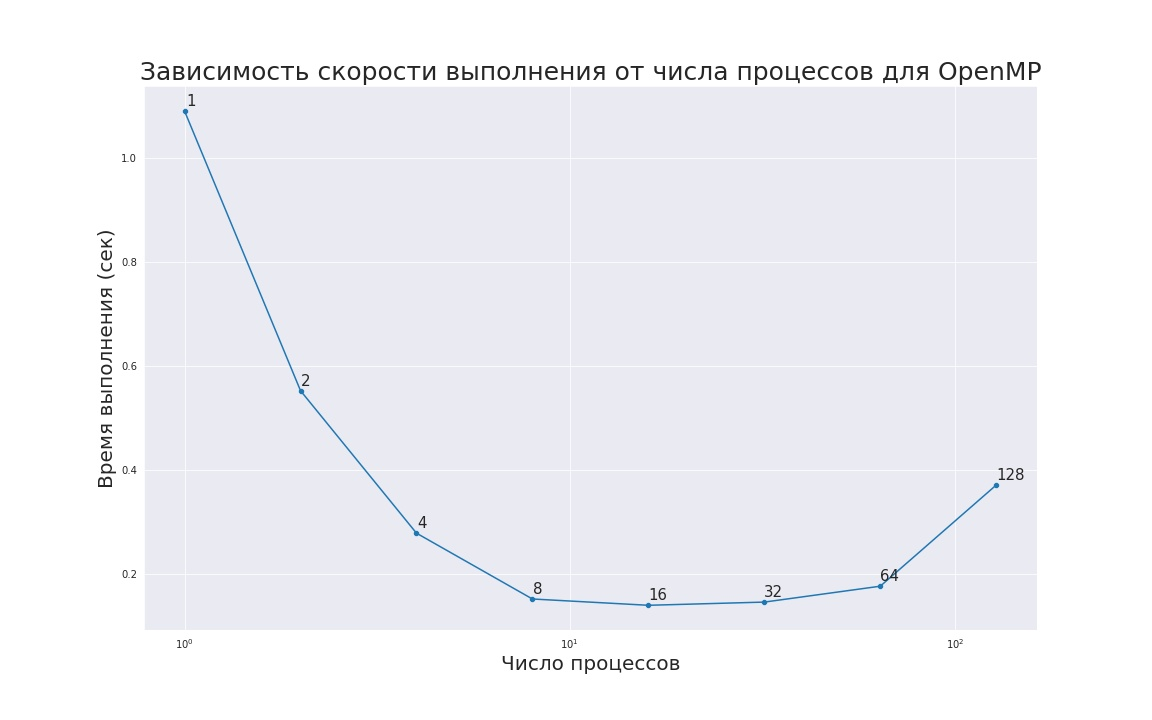
\includegraphics[width=0.9\textwidth]{images/openmp2.jpg}
\end{center}

Можно сделать наблюдение, что с ростом числа потоков увеличивается скорость работы. Однако когда процессов слишком много, наклодные расходы существенно замедляют время работы

\subsection{Скорость работы MPI}
На графике представлена зависимость скорости работы алгоритма, написанного с использованием MPI
\begin{center}
  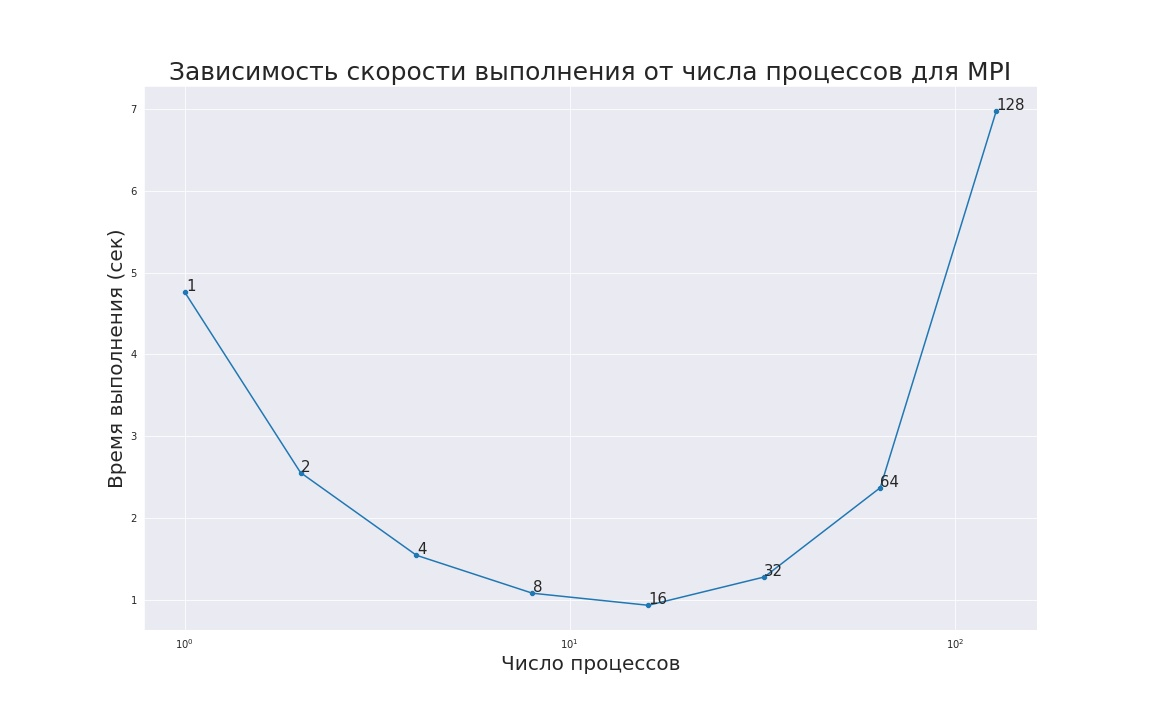
\includegraphics[width=0.9\textwidth]{images/mpi.jpg}
\end{center}

Выводы аналогичны предыдущим. Из отличий, время работы получилось в 10 раз хуже, чем для OpenMP. Также при увеличении числа потоков накладные расходы гораздо сильнее сказываются на производительности, чем в случае OpenMP.

\section{Выводы}
Оба фреймворка OpenMP и MPI позволяют ускорить программу. Однако первый из них позволяет сделать это с меньшими изменениями кода и при этом большим ускорением. С увеличением числа потоков возрастает производительность, однако при слишком большом числе потоков замедление из-за накладных расходов компенсирует полученное ускорение.

\newpage
\section{Приложения}
\import{./}{code.tex}
\end{document}